\documentclass[10pt, a4paper]{article}
\usepackage[utf8]{inputenc}
\usepackage[russian]{babel}
\usepackage[sb]{libertine}
\usepackage{a4wide}
\usepackage{listings}
\usepackage{graphicx} 

\begin{document}

\title{Отчёт по лабораторной работе №6}
\author{Окорочкова Мария, M32341}

\maketitle

\section*{1. Детали реализации каждого алгоритма.}
\subsection*{Алгоритм эксперимента № 1}
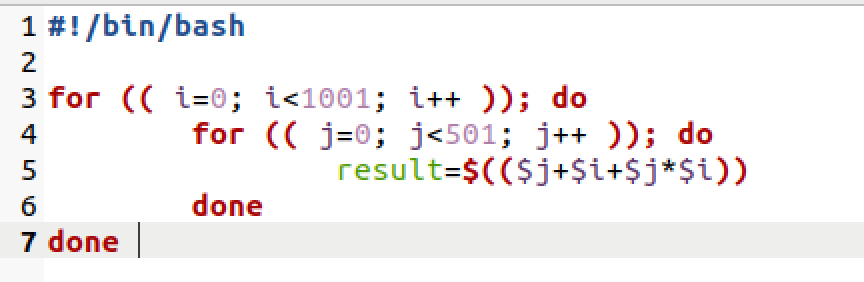
\includegraphics[scale=0.7]{scripts/algo1.png}
\subsection*{Алгоритм эксперимента № 2}
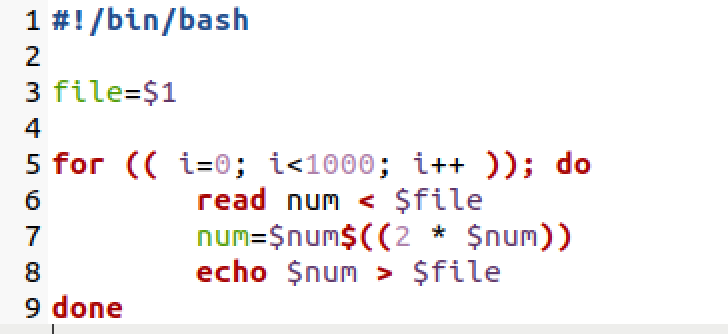
\includegraphics[scale=0.8]{scripts/algo2.png}
\subsection*{Общий скрипт запуска} 
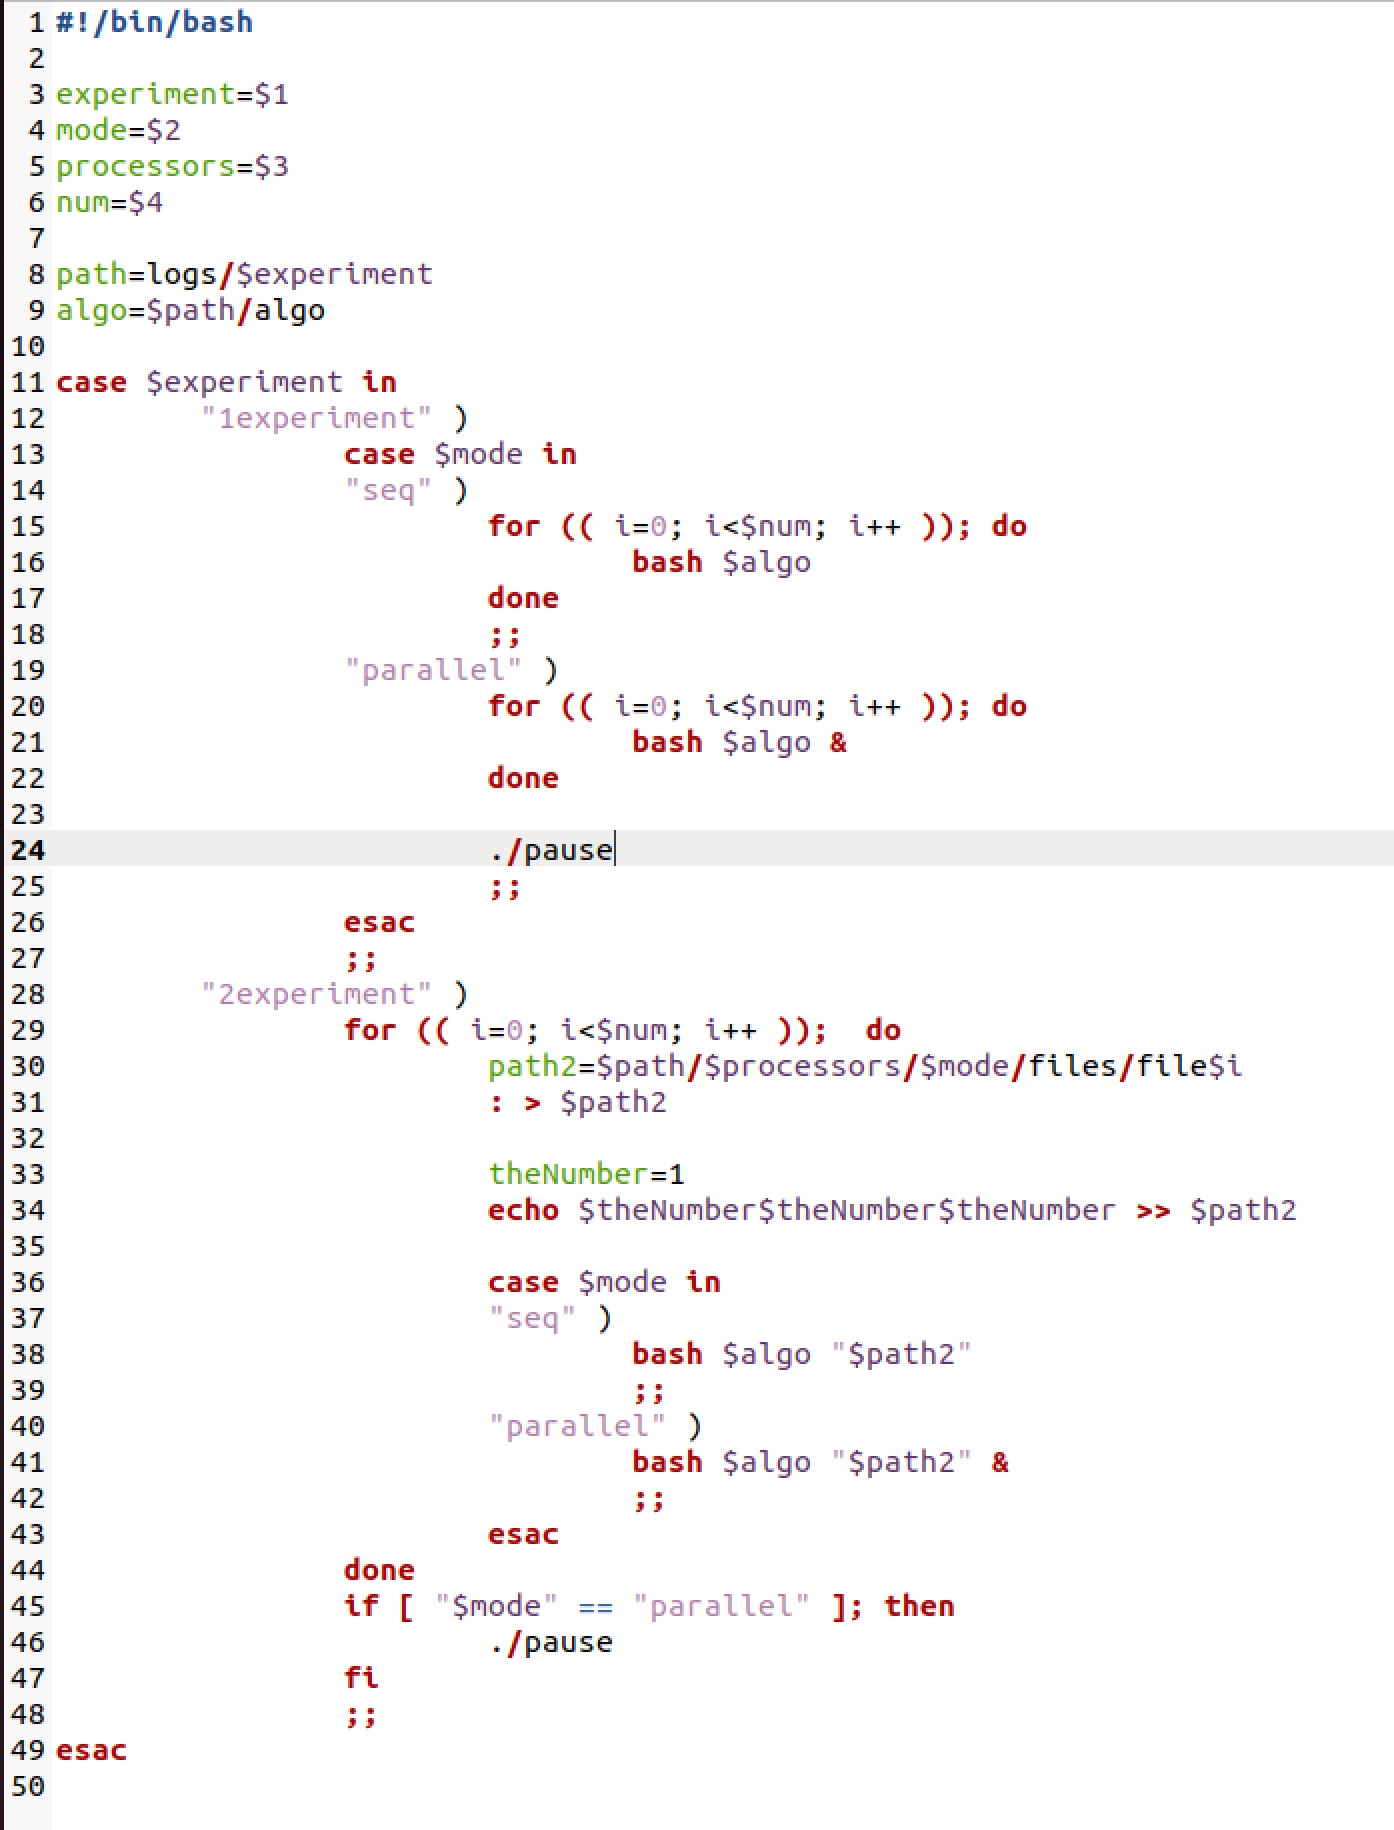
\includegraphics[scale=0.7]{scripts/launch.png}
\subsection*{Общий скрипт оценки времени алгоритма (получаем при вызове \texttt{time -p} значение параметра \texttt{real})}
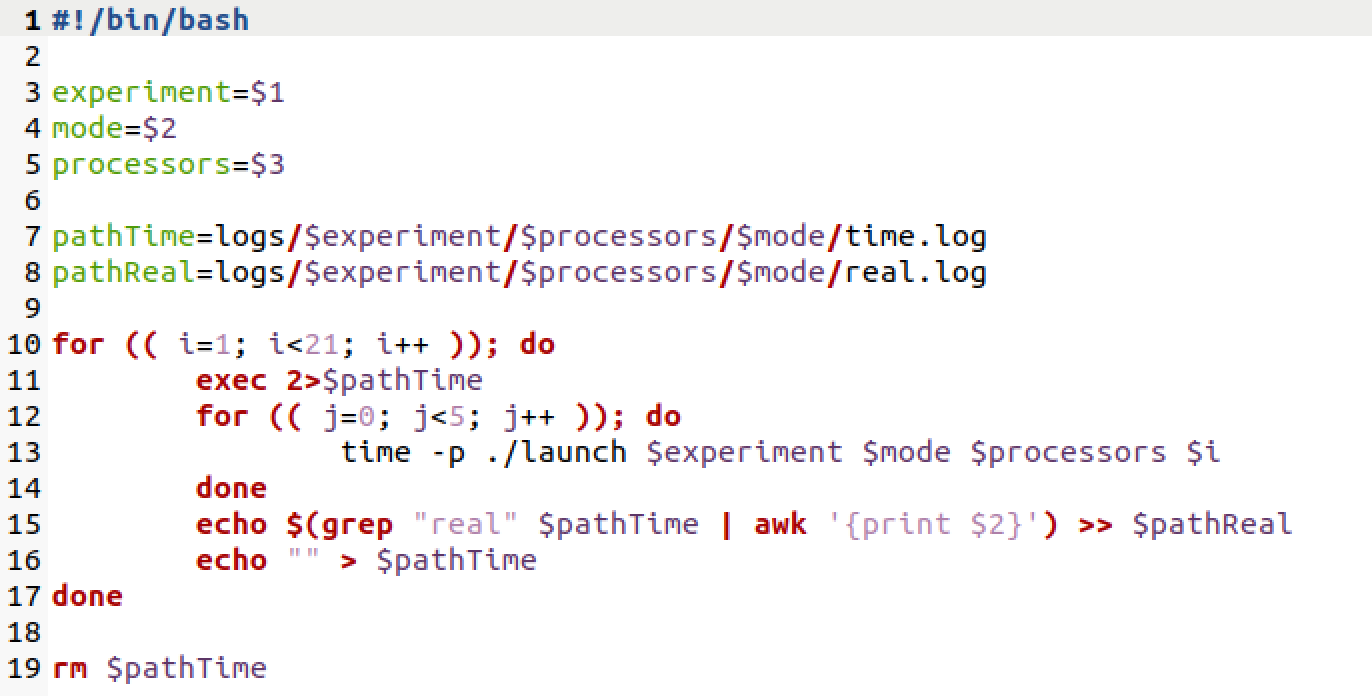
\includegraphics[scale=0.7]{scripts/pause.png}

\section*{2. Параметры.}
\subsection*{Хостовый компютер}
\begin{tabular}{|l|r|}
      \hline
    Память & 16 ГБ 2133 MHz LPDDR3 \\
      Имя процессора & 4‑ядерный процессор Intel Core i7 \\
    Скорость процессора &	2,8 GHz  \\
  Количество процессоров & 1  \\
  Общее количество ядер & 4  \\
  Кэш 2-го уровня (в каждом ядре) & 256 КБ \\
  Кэш 3-го уровня & 6 МБ \\
    \hline
\end{tabular}
\subsection*{Виртуальная машина}
\begin{tabular}{|l|r|}
      \hline
Основная память & 2048 МБ \\
Порядок загрузки & Гибкий лиск -> Оптический диск -> Жёсткий диск \\
Чипсет & PIIX3
TPM & отсутствует 
Процессор & 1 или 2 ЦП \\
Предел загрузки ЦПУ & 100\% \\
    \hline
\end{tabular}

\section*{3. Дополненные планы экспериментов.}
Запускаем скрипты и берём логи с помощью следующих команд
\begin{lstlisting}
./range 1experiment seq 1
./range 1experiment parallel 1
./range 1experiment seq 2
./range 1experiment parallel 2
./range 2experiment seq 1
./range 2experiment parallel 1
./range 2experiment seq 2
./range 2experiment parallel 2, 
\end{lstlisting}
где первый параметр -- эксперимент, второй -- способ запуска, третий -- кол-во процессоров.

К сожалению, пришлось не соблюсти условие о количестве запусков скрипта (в цикле от 1 до 20) для подсчёта среднего арифметичееского выполнения алгоритма. Дело в том, что, если запускать, как предлагается, 10 раз, то придётся потратить на выполнение работы 13-14 часов, что затруднительно. Поэтому приняла решение запускать скрипт не 10 раз, а 5.

\section*{4. Графики + комментарии.}

\subsection*{Искомое среднее время выполнения:}
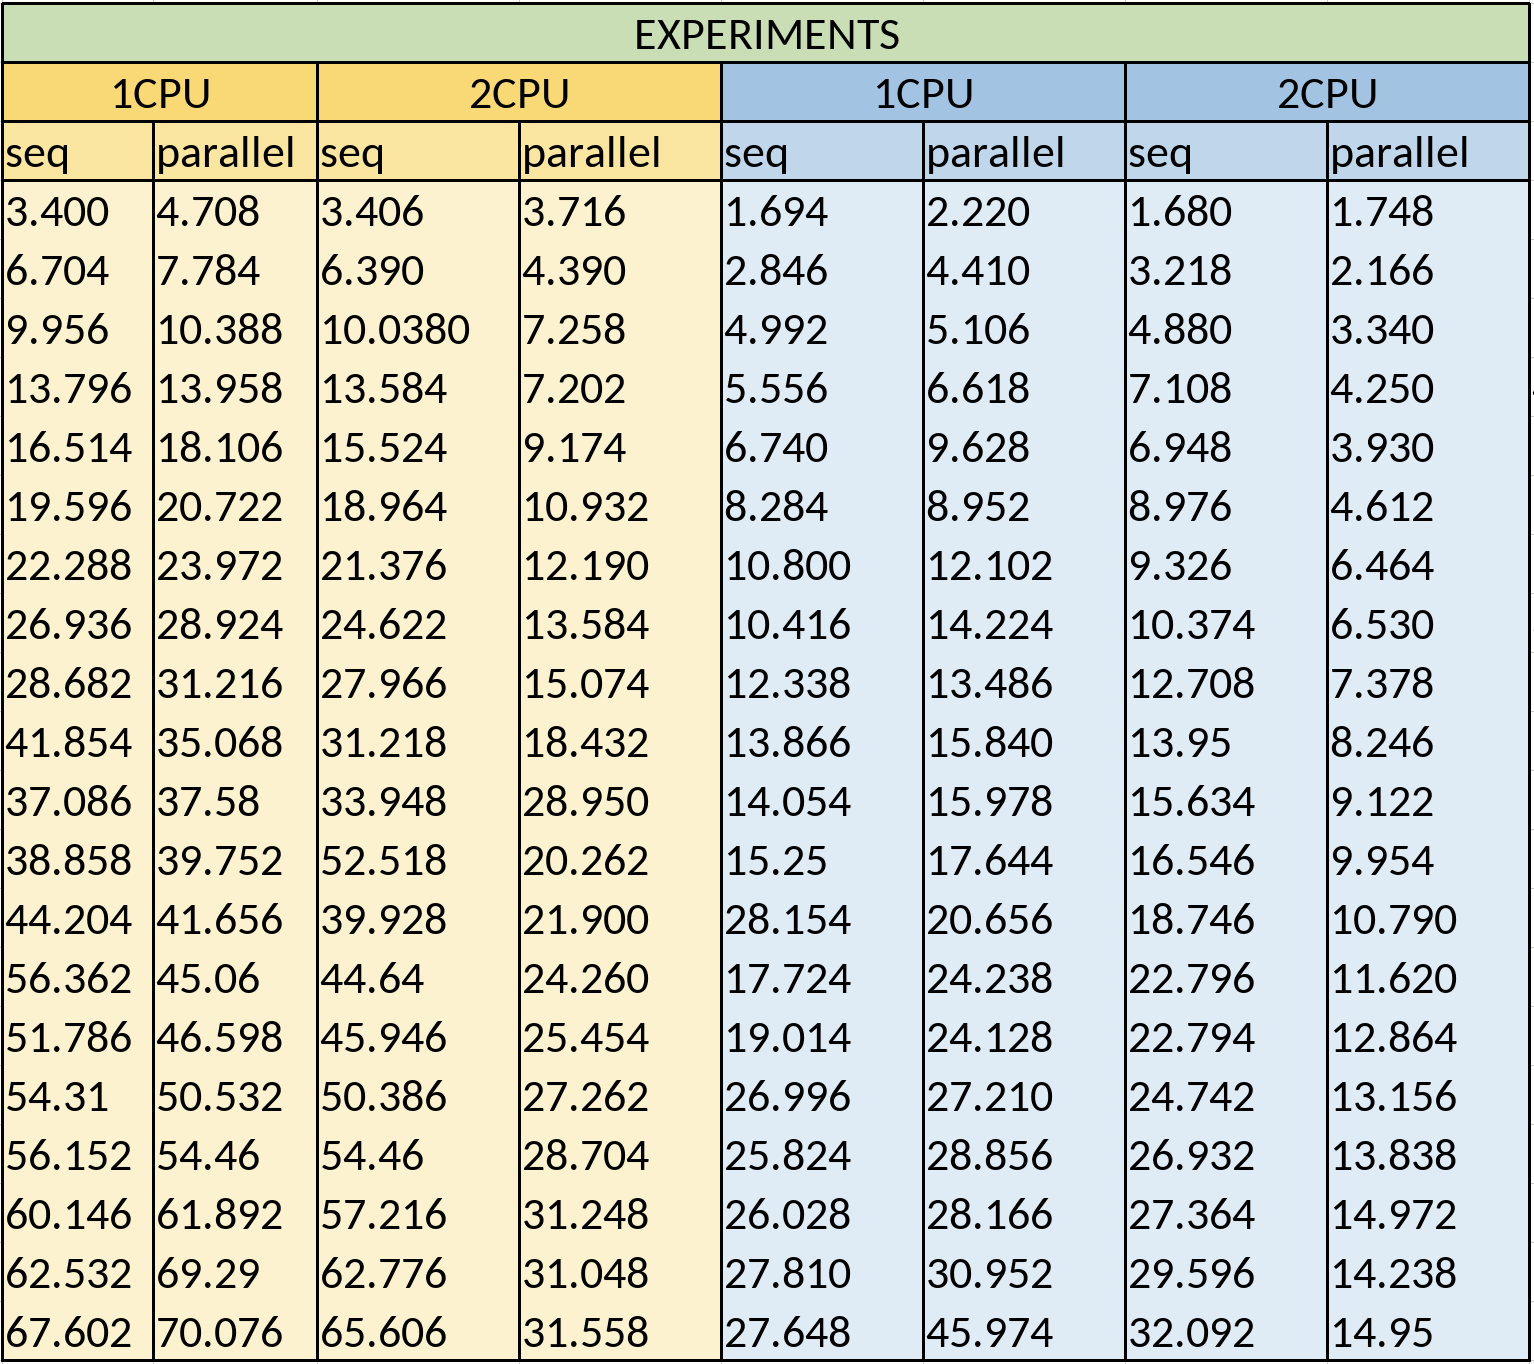
\includegraphics[scale=0.6]{table.png}

\subsection*{Эксперимент №1}
\begin{itemize}
    \item 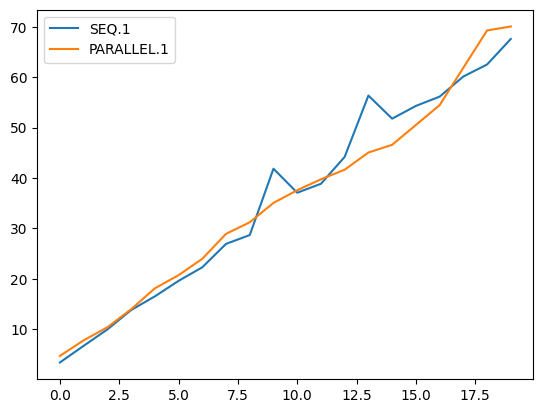
\includegraphics[scale=0.6]{graphs/1.png}
    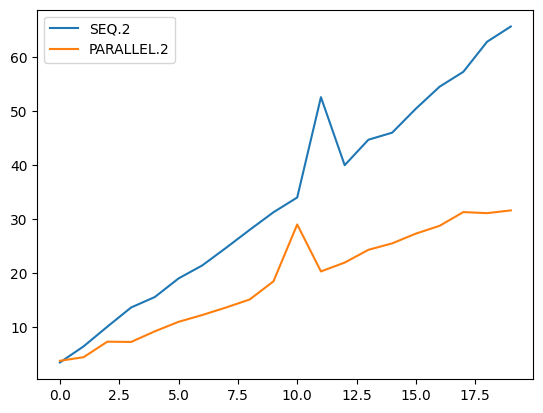
\includegraphics[scale=0.6]{graphs/2.png}

    \item 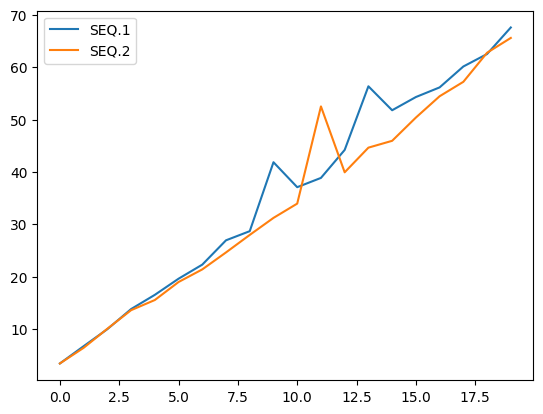
\includegraphics[scale=0.6]{graphs/3.png}
    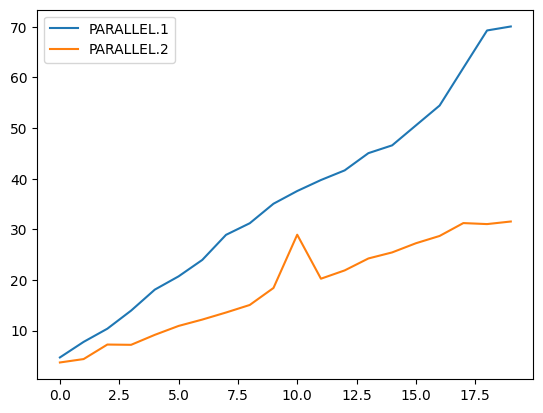
\includegraphics[scale=0.6]{graphs/4.png}
\end{itemize}

\subsection*{Эксперимент №2}
\begin{itemize}
    \item 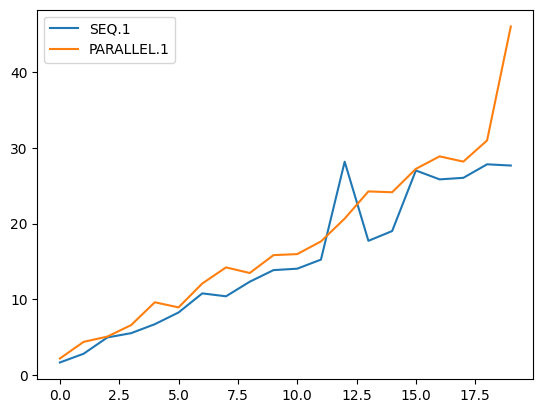
\includegraphics[scale=0.6]{graphs/5.png}
    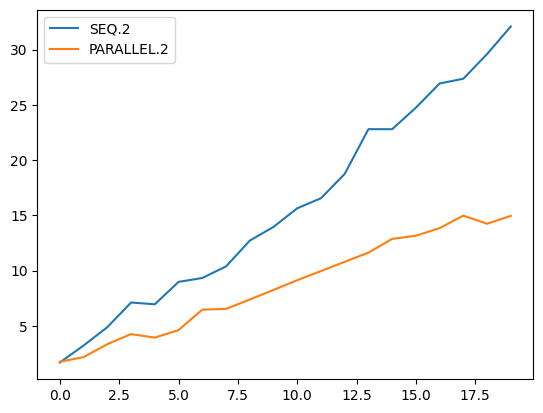
\includegraphics[scale=0.6]{graphs/6.png}

    \item 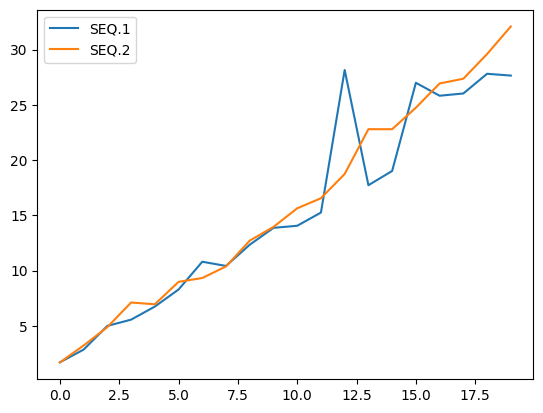
\includegraphics[scale=0.6]{graphs/7.png}
    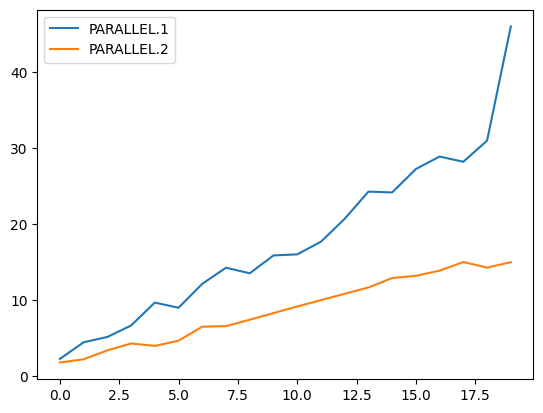
\includegraphics[scale=0.6]{graphs/8.png}
\end{itemize}

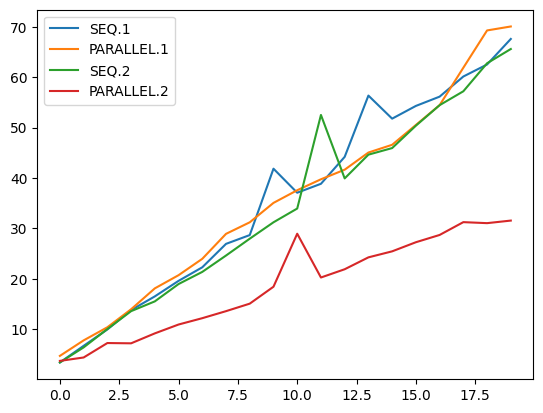
\includegraphics{graphs/9.png}


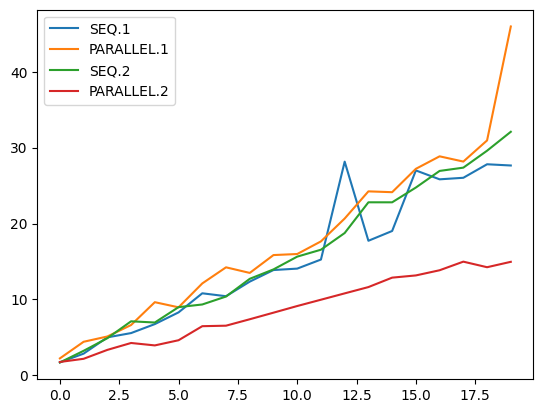
\includegraphics{graphs/10.png}

\subsection*{Комментарии: }
\begin{itemize}
    \item Один процессор, сравнение последовательного и параллельного вызовов: значительной разницы по времени выполнения не наблюдается.
    \item Два процессора, сравнение последовательного и параллельного вызовов: выражается более быстрое выполнение при параллельном вызове. 
    \item Cравнение последовательных вызовов при разном кол-ве процессоров: значительной разницы по времени выполнения не наблюдается.
    \item Cравнение параллельных вызовов при разном кол-ве процессоров: выражается более быстрое выполнение при двух процессорах.
    \item Больше всего времени тратится на параллельные вызовы скрипта при одном потоке, а меньше всего -- на параллельные вызовы скрипта при двух потоках. 
    \item Характер поведения времени первого и второго экспериментов крайне схож. 
    \item Пристуствует некоторая погрешность ("скачки" на графиках).
\end{itemize}

\section*{5. Выводы:}
\begin{itemize}
    \item Эффективнее, конечно, использовать два потока(процессора), ведь тогда нагрузка будет распределяться равномерно. 
    \item Параллельный способ запусков следует использовать при выполнении скрипта на двух процессорах/потоках, так быстрее. Опять же, играет роль распредление нагрузки.
    \item Последовательный способ запусков следует использовать при выполнении скрипта на одном процессоре/потоке, так быстрее. Параллельность на одном процессоре будет только мешать. 
    \item Эксперимент №1 с выполнением вычислительно сложных задач выполняется медленее эксперимента № 2 с выполнением задач с большими объемами считываемых и сохраняемых данных, что ожидаемо.
\end{itemize}

\end{document}






